\chapter{Introduction} \label{introduction}

The Roa Logic AHB-Lite Timer IP is a fully parameterized soft IP
implementing a user-defined number of timers and functions as specified
by the RISC-V Privileged 1.9.1 specification.

The IP features an AHB-Lite Slave interface, with all signals defined in
the \emph{AMBA 3 AHB-Lite v1.0} specifications fully supported,
supporting a single AHB-Lite based host connection. Bus address \& data
widths as well as the number of timers supported are specified via
parameters.

The timebase of the timers is derived from the AHB-Lite bus clock,
scaled down by a programmable value.

The module features a single Interrupt output which is asserted whenever
an enabled timer is triggered

\begin{figure}[tbh]
	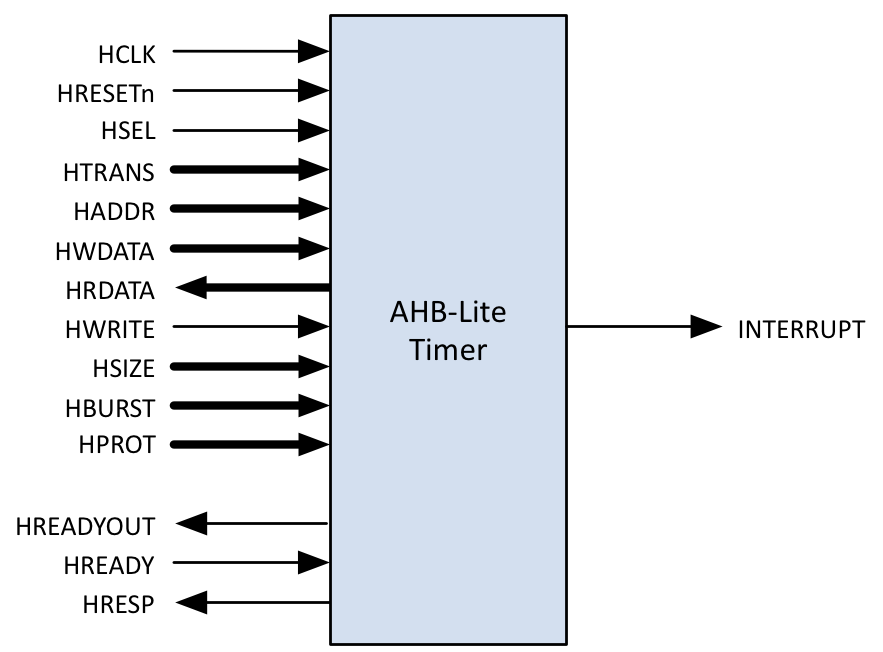
\includegraphics{assets/img/AHB-Lite-Timer-sig.png}
	\caption{AHB-Lite Timer}
	\label{fig:ahb-lite-timer-sig}
\end{figure}

\section{Features}\label{features}

\begin{itemize}
\item
  AHB-Lite Interface with programmable address and data width
\item
  User defined number of counters (Up to 32)
\item
  Programmable time base derived from AHB-Lite bus clock
\end{itemize}